\section{Discussion}
\label{sec:discussion}

\subsection{Modelisation of the \SD data for \spinhole pinhole}

Based on the work from \cite{moffat}, the \SD telescope PSF can be modelized as a moffat distribution. When shooting with the \spinhole pinhole inside the \SD telescope, the flux $F(r, \lambda)$ measured in the CDD with aperture photometry at a radius $r$ and a wavelength $\lambda$, can be modelized as: 

\begin{equation}
F(r, \lambda) = \frac{A(\lambda) \times M(r, \lambda) + \Kghostfit(r, \lambda)}{1 + \Kghostfit(r \rightarrow +\infty, \lambda)} + \bkg(r, \lambda),
\label{eq:moffat_model}
\end{equation}
with $A(\lambda)$ the total amplitude, $\Kghostfit(r, \lambda)$ the relative contribution of the 1\up{st} order ghost to $A(\lambda)$, $\bkg(r, \lambda)$ the contribution of the background and $M(r, \lambda)$ the moffat distribution defined as:

\begin{equation}
M(r, \lambda)= \left( 1+\frac{r^2}{\alpha(\lambda)^2} \right)^{-\beta(\lambda)},
\end{equation}
with $\alpha(\lambda)$ and $\beta(\lambda)$ the parameters of the Moffat distribution. The flux is normalized by $(1 + \Kghostfit(r \rightarrow +\infty, \lambda))$ so its infinite integral is equal to the maximum amplitude $A(\lambda)$. 

The core of the PSF is actually more complex than a moffat distribution because of the intrisinc shape of the CBP output. However the tail of the PSF should not be impacted by this, and is expected to behave like a Moffat distribution. 
The model is fitted on aperture photometry for a radius $r=\SI{20.9}{pixels}$, and then annulus of external radius from \SI{24.9}{pixels} to \SI{419.1}{pixels}. These radius are regularly spaced on a logarithm scale, as shown in Figure~\ref{fig:apertures_fit}. To take in account $\Kghostfit(r, \lambda)$, an additive value is set free for every annulus that contains a ghost contribution. The parameters $A(\lambda)$, $\alpha(\lambda)$, $\beta(\lambda)$, $\Kghostfit(\lambda)$ and $\bkg(\lambda)$ are adjusted with the \spinhole pinhole dataset No.~8 from Table~\ref{tab:schedule}. 

\begin{figure}[h]
     \centering
     \resizebox{\hsize}{!}{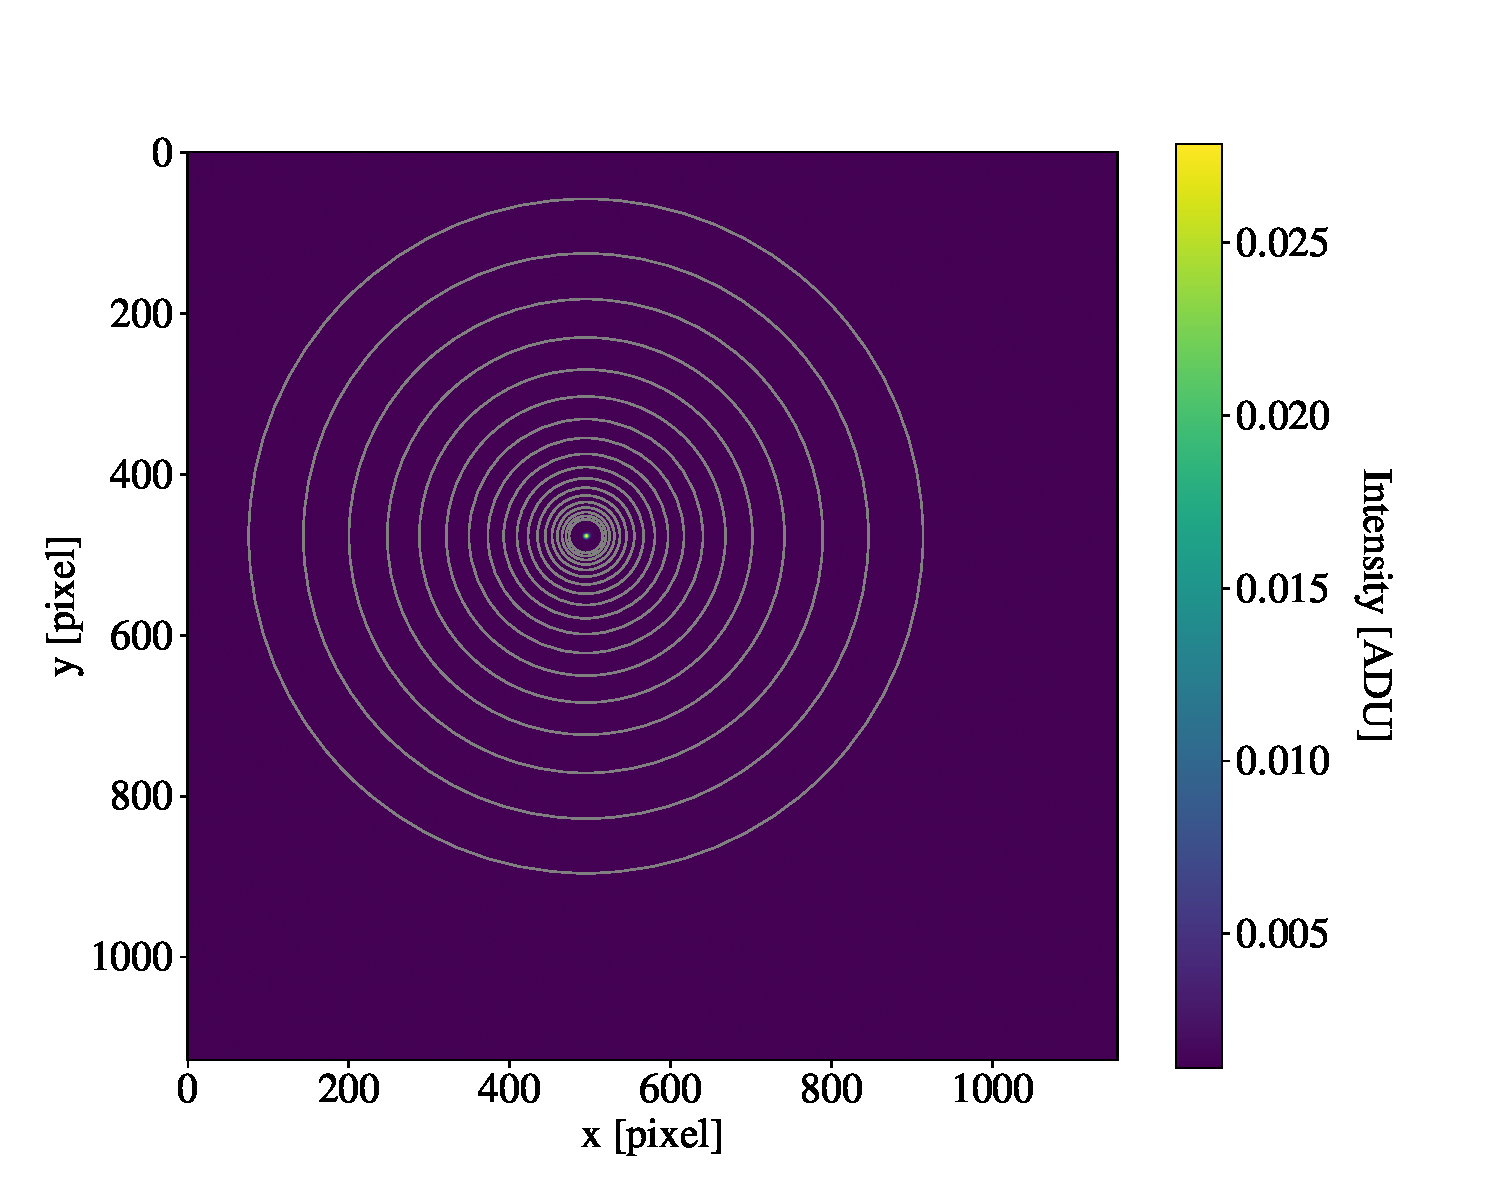
\includegraphics{fig/apertures_fit.pdf}}
     \caption{Image of the \spinhole observed with the \SD camera at \SI{400}{\nano\meter}. The circles corresponds to the radius used to adjust the parameters of Equation~\ref{eq:moffat_model}.}
     \label{fig:apertures_fit}
    %~/stardice/analysis/cbp_paper/total_fluxes/jax_fit.ipynb
\end{figure}

The evolution of the Moffat distribution is expected to be smooth with respect to wavelength. So the parameters $\alpha(\lambda)$ and $\beta(\lambda)$ are developed on a B-spline basis with 20 wavelength nodes regularly spaced between \SI{350}{\nano\meter} to \SI{1100}{\nano\meter}. The same goes for the parameters $G_1(\lambda)$ as it corresponds to light coming from reflections on surfaces in the optical path. The results of this fit is shown Figure~\ref{fig:result_params}. The bottom panel corresponds to the aperture correction that is needed to apply to the aperture photometry measurement. It is around 2\% below \SI{950}{\nano\meter}, and increase by one order of magnitude in the infrared. This increase is correlated with the variation of the Moffat parameters $\alpha$ and $\beta$, showing that the PSF is drastically changing in the near infrared. This issue is discussed in more details section \ref{sec:ir}. The third panel show a constant background against wavelength, at a mean of \SI{0.27}{ADU/pixel}.

\begin{figure}[h]
     \centering
     \resizebox{\hsize}{!}{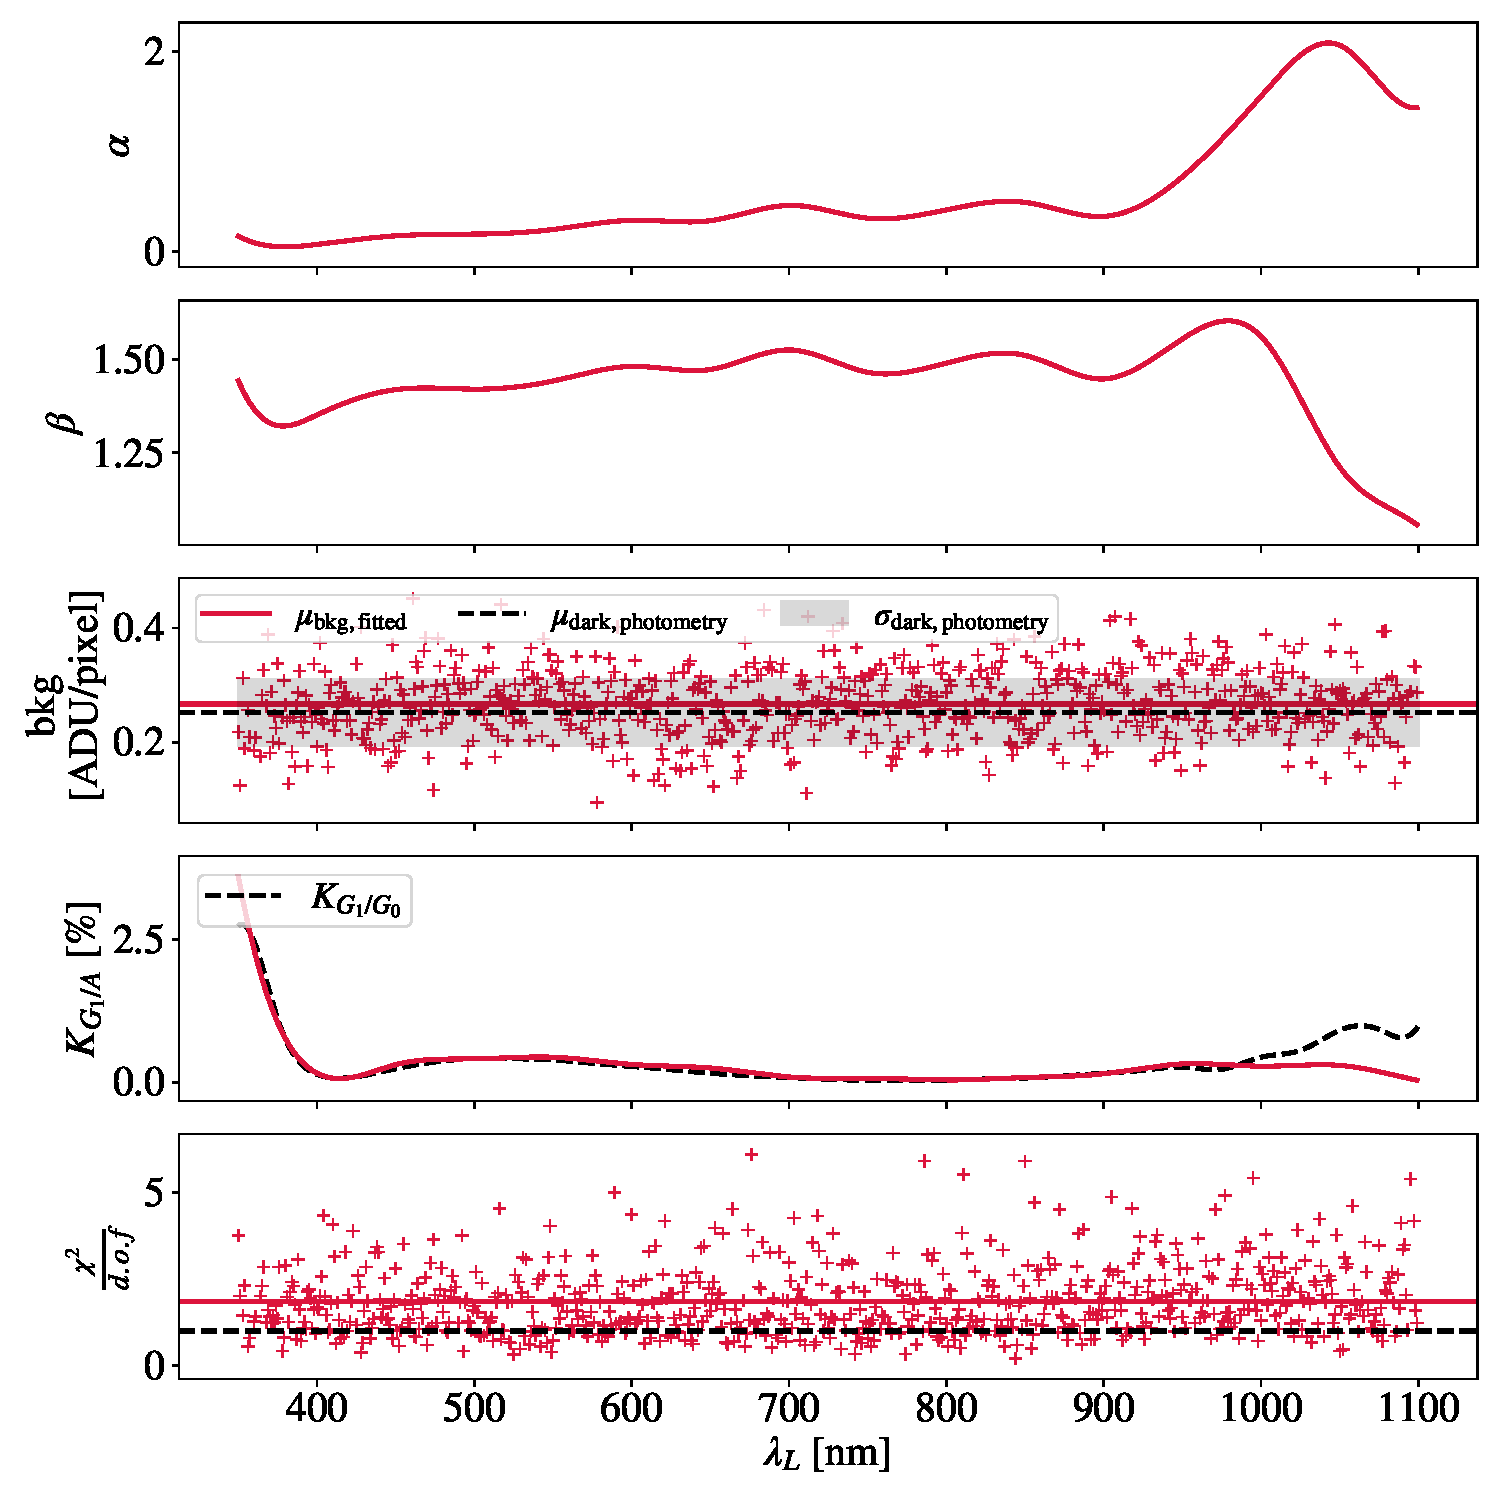
\includegraphics{fig/result_params.pdf}}
     \caption{Result of the model of Equation~\ref{eq:moffat_model} adjusted on the \spinhole pinhole dataset No.~8 from Table~\ref{tab:schedule}. The first and second panel represent respectively the $\alpha$ and $\beta$ parameters from the Moffat distribution. The third panel represent the background contribution per pixel. The fourth panel represent $\Kghostfit$, and $\Kghost$ for which the measurement has been detailed in section \ref{sec:ghost}. The fifth panel represent the missing fraction when measuring the \spinhole with aperture photometry compared to the total amplitude fitted $A$.}
     \label{fig:result_params}
    %~/stardice/analysis/cbp_paper/total_fluxes/jax_fit.ipynb
\end{figure}




